\chapter{Magnetometer Operation\label{ch:characterization}}

In this Chapter I describe the different ways in which the
magnetometer was operated.  Some of these modes of operation were
applied to furhter experiments, which are reported in
Chapter~\ref{ch:results}.  Some of the modes were simply used to
perform a basic characterization of the magnetometer and to compare
with the results of other groups which were discussed in the
Literature Review in Chapter~\ref{ch:magnetometry}.

The main purpose of this Chapter is to give an overview of the many
parameters which can affect the performance of the magnetometer.
Chapter~\ref{ch:results} goes into further detail on studies of
specific performance metrics under modification of additional
parameters.

The main operation modes of the magnetometer reported in this Chapter
are:
\begin{itemize}
\item Near-zero-field operation.  In this mode, the magnetic field
  must be swept in order to calibrate the magnetometer.  The dynamic
  range of the magnetometer in this case is $|B_z|\lesssim 0.2$~nT.
\item Amplitude modulated NMOR, which itself was used in two distinct modes:
\begin{itemize}
\item Continuously pumped (a.k.a.~forced oscillation) mode.  In this
  mode, the amplitude of the pump beam was modulated continuously and
  the optical rotation signal was demodulated resonantly at the same
  frequency.
\item Free-induction decay (FID) mode.  In this mode, the amplitude of
  the pump beam is modulated for a time and then switched off.  The
  oscillation frequency of the optical rotation signal is then
  measured non-resonantly.
\end{itemize}
In these modes, the magnetometer was generally operated at 0.2~$\mu$T
or 1.0~$\mu$T, which is of considerably more relevance to the nEDM
experiment.
\end{itemize}
In Chapter~\ref{ch:results}, most of the measurements will relate to
our studies using FID mode.  The exception is that some degaussing
studies will be done near zero field and hence will use that mode.


\section{NMOR near zero field and degaussing studies}

During this measurement the pump beam was switched off and the probe
beam is used as its own pump (see
Section~\ref{sec:something-in-chapter-3}).

I used the magnetometer in this mode to study the function of the
degaussing system described in
Section~\ref{sec:Degaussing}.

The experiment was carried out as follows:
\begin{enumerate}
\item The laser beam was tuned for maximum optical rotation and
  stabilized using the DAVLL system.  The beam power was $\sim
  20~\mu$W.
\item Optical rotation of the probe beam was monitored throughout the
  experiment via an oscilloscope monitoring the differential
  photodiode signal.
\item The innermost magnetic shield was degaussed with various
  parameters for the sequence.  The operation of the degaussing
  circuit was described in Section~\ref{sec:Degaussing}.  After
  completing the degaussing sequence a switch is opened to
  electrically isolate the degaussing coil.
\item The magnetic field along the $z$-direction (defined in
  Section~\ref{sec:Internal coil}) is swept in order to calibrate the
  differential photodiode signal as a function of applied $B_z$.  In
  this way the initial magnetic field after degaussing may be deduced.
\end{enumerate}
%In this case,  at first degaussing the shields that surround the vapour cell is done in order to cancel background B-field.A function generator is used to drive the degaussing coil. After completing a degaussing sequence switch is opened to electrically disconnect the degaussing coil from experimental setup. Then B-field ramp is started and NMOR signal is observed through a oscilloscope which  connected to balance photodiode output. The magnetic field sweeping is done in a triangle wave. In 
Fig.~\ref{fig:TUNE} displays the sequence of measurement events in
time, along with the differential photodiode signal (in Volts), which
is proportional to optical rotation.  Also shown is a voltage applied
to the $z$-coil with a 10~k$\Omega$ resistor in series which dominates
the resistance of the circuit.  Recall that the coil constant of the
$z$-coil is $\sim 48$~nT/mA (see Section~\ref{sec:Internal coil}).
The sweep range of this trace is therefore
% (0.8~V)/(10000~Ohm)/*48~nT/mA = 3.84 nT ???  It would be good to
% write the correct calibration constant in the part of the thesis
% where this coil is describe (probably somewhere in Chapter 3).
1.9~nT peak to peak.

In the first section of the oscilloscope trace, the impact of the
degaussing procedure inducing noise in the optical rotation signal can
be seen.  The next section involves the ramping down of a variable
resistor, followed by opening the switch to isolate the degaussing
coil.  Then the magnetic field $B_z$ is swept and the characteristic
dispersive Lorentzian shape of NMOR is observed.

\begin{figure}%[h]
\centering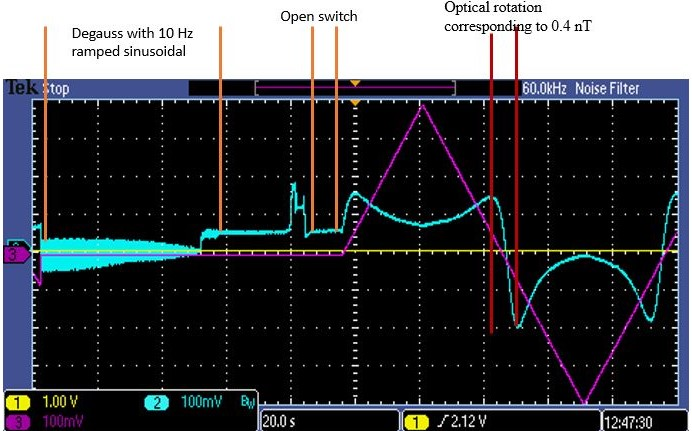
\includegraphics[width=0.7\linewidth]{figures/scope_trace_of_field_sweeping}
\caption{Oscilloscope trace of measurement OR near zero field. The
  purple curve shows the voltage across the 10~k$\Omega$ resistor in
  series with the $z$-coil, from which the magnetic field ramp of
  1.9~nT peak to peak can be deduced.  The blue trace indicates the
  differential photodiode signal which is proportional to the optical
  rotation.  The left side of the traces show the impact of the
  degaussing procedure, while the right side shows the calibration
  procedure.\label{fig:TUNE} }
\end{figure}


In this measurement NMOR signal is used to determine effectiveness of
degaussing procedure. After the degaussing procedure the observed OR
signal is non-zero while the applied field $B_z$ was zero which
indicates the existence of a remnant field.  The effect of degaussing
parameters sensed by the magnetometer is discussed further in
Section~\ref{sec:degaussing}.


% We need to have this table somewhere, but I think it needs to be in
% the section where you talk about degaussing.

%\begin{table}%[h]
%\centering
%\begin{tabular}{|l|l|}
%\hline
%\textbf{SETTING}    & \textbf{VALUE} \\
%\hline
%Function generator &   \\
%\hline
%Frequency &  10 Hz   \\
%Sample rate    &  10000 sample/sec  \\
%Amplitude   &   10 V \\
%Offset  &       0 V  \\
%\hline
%\end{tabular}
%\caption{Setting for degaussing \label{table:degaussing setting}}
%\end{table}

Fig.~\ref{fig:near zero field} shows an example of the calibration of
the differential photodiode signal to the field applied by the
$z$-coil, for data where the degaussing part of the sequence have been
removed.  The field is calibrated to the voltage signal as described
above.  In Fig.~\ref{fig:near zero field}, the data have been fitted
to a dispersive Lorentzian shape given by the function
\begin{equation}
\mathrm{Signal~(V)}=\frac{A(B-B_0)}{somefunctionthatMoushumifillsin}
\end{equation}
where $A$, $B_0$, $a$, and $o$ are fit parameters.  A key measure of
magnetometer performance is the valley-to-peak distance, which in this
case is about $\Delta B=\frac{2}{a}=0.49$~nT.  The other key measure
in this case is the deduced field at zero crossing given by the fit
parameter $B_0=0.019$~nT.  Thus, after degaussing, a remanent field of
19~pT is found.  This is only the on-axis field.  It is possible that
transverse fields can be larger, and these tend to make the width
$\Delta B$ of the zero-field curve larger.

\begin{figure}[h]
\centering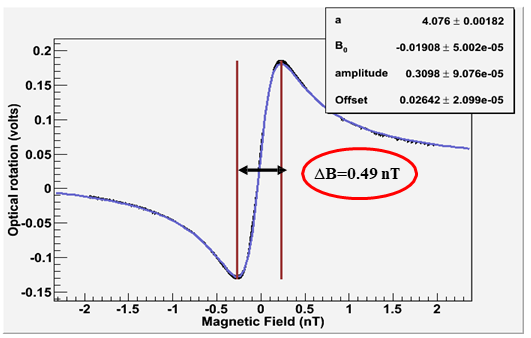
\includegraphics[width=0.7\linewidth]{figures/near_zero_field}
\caption{Optical rotation as a function of magnetic field applied
  along the direction of the laser beam. The signal looks like a pure
  dispersive Lorentzian curve. The measured resonance width is 0.49~nT
  and the measured remanent field is 0.019~nT.\label{fig:near zero
    field}}
\end{figure}

In order to determine the sensitivity, a magnetometer can be operated
in different modes. Most of them found its application during the time
this Master's thesis was prepared. Although main focus of this work
was to study magnetometer performance in Free Induction Decay (FID)
mode.

\section{Amplitude Modulated NMOR:  Forced Oscillation Mode}

In this forced-oscillation measurement scheme the pump beam amplitude
is modulated and the differential photodiode signal is demodulated at
the same frequency $\Omega_m$ using a lock-in amplifier.  The
modulation/demodulation frequency is near twice the Larmor frequency
of the atoms in the magnetic field.

In the first instance, we tried keeping the frequency constant and
sweeping the magnetic field.  We can then determine the resonant field
by fitting the resonance lineshape.  The disadvantage of this method
is that the field must be changed in order to measure it.  {\bf An
  example of this might be shown in Fig.~\ref{fig:AMORmaybeidontknow},
  or it might not be.  Really, it is impossible to tell.}

\begin{figure}[h]
\centering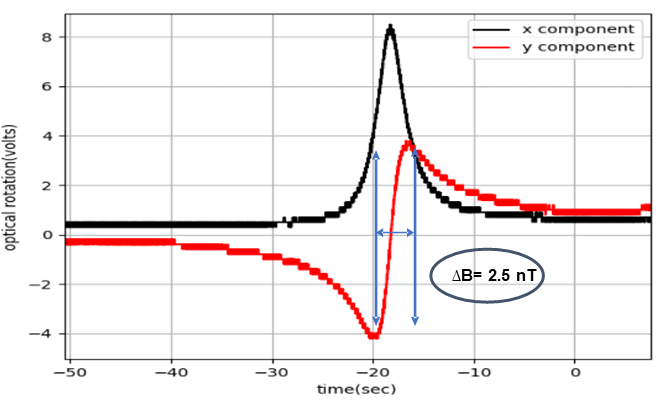
\includegraphics[width=0.7\linewidth]{figures/AM_NMOR}
\caption{\bf The rest of this figure caption might be totally
  false... AMOR resonance signal with a 5 cm cell containing natural
  Rb.  Data was acquired by using a balanced photodiode which
  demodulated through lock-in amplifier as the frequency is swept
  slowly near 9.37~kHz.  The parameters of the sweep are shown in
  Table~\ref{tab:freqsweep} and are discussed further in the text. The
  observed resonance width, when translated from frequency into field,
  is 2.5~nT.\label{fig:AMORmaybeidontknow}}
\end{figure} 

A better way to measure the field without having to change it is to
sweep the modulation/demodulation frequency instead.  The resonant
frequency then gives a determination of the field (when
$\Omega_m=2\Omega_L$)

\begin{figure}[h]
\centering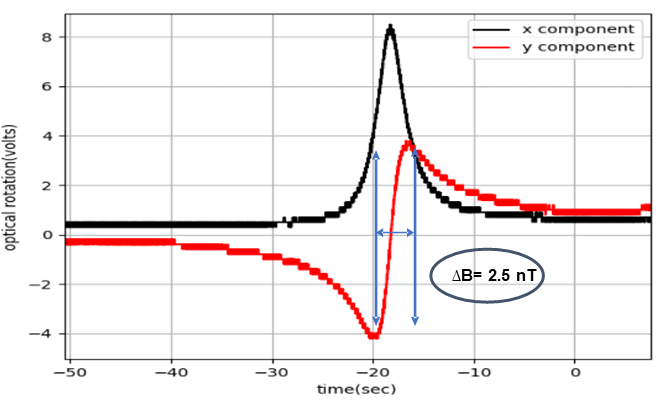
\includegraphics[width=0.7\linewidth]{figures/AM_NMOR}
\caption{\bf I do not know what this figure is, and so here is what
  I'm guessing that it might be: AMOR resonance signal with a 5 cm
  cell containing natural Rb.  Data was acquired by using a balanced
  photodiode which demodulated through lock-in amplifier as the
  frequency is swept slowly near 9.37~kHz.  The parameters of the
  sweep are shown in Table~\ref{tab:freqsweep} and are discussed
  further in the text. The observed resonance width, when translated
  from frequency into field, is 2.5~nT.\label{fig:AMOR}}
\end{figure} 

Fig.~\ref{fig:AMOR} {\bf potentially, maybe, and if it doesn't we
  should find the figure that does show this, since you included the
  table below which relates to the data that may or may not be
  presented in the figure but should be} shows a measurement of the
in-phase and quadrature signals measured while the frequency is swept
very slowly.  The parameters of this mode of operation, particularly
of the slow frequency modulation, are shown in
Table~\ref{tab:freqsweep}.

\begin{table}%[h]
\centering
\begin{tabular}{|l |l|}
\hline

\textbf{ SETTING}    & \textbf{VALUE} \\
\hline
Function generator &   \\
\hline
Frequency & 9.37kHz   \\

Waveform    &  Square  \\

Amplitude   &  $1V_{pp}$  \\
Offset  &       500 mV  \\
Duty cycle       &    $1\%$ \\
Frequency Deviation     &   40 Hz  \\
FM Frequency     &   100 mHz  \\
modulation waveform      &    Triangle \\
Amplitude modulation & On \\
\hline
Lock-in amplifier &     \\
\hline
Lock in frequency     & 9.37 KHz \\
Time constant     &  $300\mu s$ \\
Sensitivity      &  100mV  \\
\hline
\end{tabular}
\caption{Setting for AM NMOR at $1\mu$T field {\bf which may or may
    not correspond to any other data showed in any other figure of
    these thesis.  All other parameters of the measurement are
    apparently unknown.}.\label{tab:freqsweep}}
\end{table}

Fig.~\ref{fig:AMOR} shows the characteristic dispersive and absorptive
shapes in the in-phase and quadrature signals, respectively.  This is
in good agreement with expectation.  The quality of the magnetometer
is again characterized by the peak-to-valley distance in frequency,
which, when translated to field corresponds to a width of 2.5~nT.

A drawback of this mode of operation is that the drive frequency is
constantly changing, so that each data point for optical rotation
represents a range of drive frequencies that were sampled within the
lock-in time constant.  A more robust method involves selecting
particular frequencies in series and then fitting to determine the
resonant frequency, as done in Ref.~\cite{bib:michithesis}.  I tried
this method also, which I call a forced-oscillation scan.

For this forced-oscillation scan a frequency range and frequency
increments are entered into a custom python code. Via a USB
connection, the function generator is set to the appropriate
frequencies, driving the pump modulation of the magnetometer. The
frequencies are taken by the lock-in amplifier as a reference signal
as well as the differential output of the polarimeter board which is
demodulated at the reference frequency. The resulting in-phase (X) and
quadrature (Y) outputs are collected by the python code via GPIB.  A
settling time of at least 5 lock-in time constants ensures that no
memory of the previous frequency is retained by the lock-in amplifier.
\begin{figure}[h]
\centering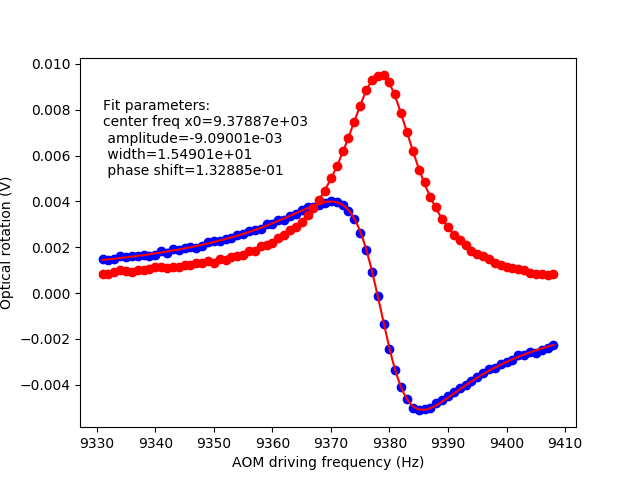
\includegraphics[width=0.4\linewidth]{figures/FM_NMOR}
\caption{Optical rotation vs. forced oscillation frequency...{\bf with
    a set of otherwise unknown parameters being used.  Also this
    figure is never referred to in the text, apparently.}}
\end{figure}

% Refer to appropriate Section of Chapter 2, if you want to make this
% statement.

%The quadrature components arise because exactly on resonance, the
%aligned atoms produce maximum optical rotation when the alignment
%axis is at an angle of $ \pi/4$ to the direction of the light
%polarization.

%Study NMOR signal by sweeping resonance frequency with amplitude
%modulated light.

%The magnetometer can be run as a forced oscillator, where a frequency
%generator is used to sweep the frequency of the laser amplitude
%modulator through the NMOR resonance. In this case the applied
%magnetic field~($B_z$) remains fixed during a measurement cycle
%(pumping and probing).
%The experimental setup for this measurement
%scheme remains almost same as for AM NMOR.

{\bf Fig.~\ref{fig:FMOR} shows something, but I do not know what.
  Below is my best guess as to what is displayed in
  Fig.~\ref{fig:FMOR}.}

\begin{figure}[h]
\centering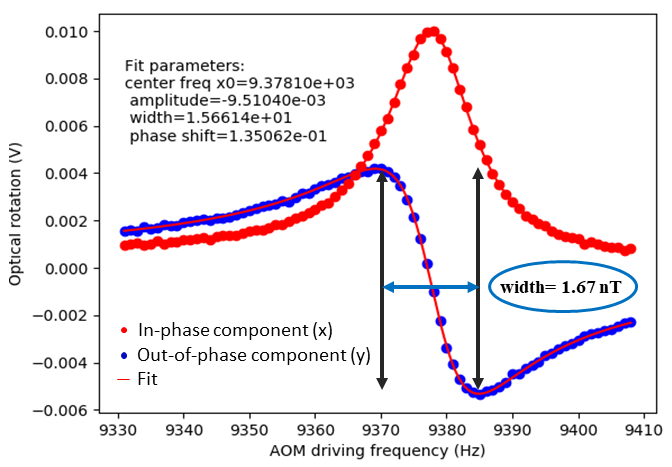
\includegraphics[width=0.5\linewidth]{figures/FM_modulation}
\caption{Demodulated components of the optical rotation, as a function
  of the forced-oscillation frequency.  NMOR resonance recorded with
  the 5 cm natural Rubidium cell, square-wave $100\%$ modulation of 1
  duty cycle. The $X$ component {\bf does not quite} reaches its
  maximum and the y component {\bf does not quite} have its zero
  crossing at $\Omega_m=2\Omega_L$ {\bf because of $\phi$}.  In this
  case the measured resonance width is 1.67~nT {\bf when translated
    from a frequency into a magnetic field???  It says a frequency, in
    the figure?  Lines drawn on the figure apparently do not line up
    with anything, and are meant to distract the
    reader?  I recommend to fix this figure.}.\label{fig:FMOR}}
\end{figure} 

The applied magnetic field was about 1~$\mu$T directed along light
propagation direction.  {\bf I think that this sentence is true.}

The measurement was taken by driving an Agilent 33522A function
generator to different modulation frequencies in order to find the
resonance frequency of the given Rb oscillator. The modulation
waveform is a square wave with a duty cycle of 1\%. Since our pump
beam is linearly polarized, a modulation at 2$\Omega_{L}$ is necessary
because of the two fold symmetry of alignment state. The typical range
of drive frequency is 9.31 KHz to 9.409 kHz for 1~$\mu$T field. An
unmodulated linearly polarized probe beam is used to analyze the spin
response. While the magnetometer response was recorded with a lock-in
amplifier, which is connected to balanced photodiode output,
demodulating the signal at the drive frequency of the atomic
oscillator.

{\bf The new things that I think I learned from this paragraph:}
\begin{itemize}
\item The duty cycle of the pump beam was 1\%.
\item The range of drive frequencies used in Fig.~\ref{fig:FMOR} was
  9.31 kHz to 9.409 kHz.
\end{itemize}


The center of the resonance is used to determine the Larmor frequency
and hence the magnetic field.  Fig.~\ref{fig:FMOR} shows the resonance
scan where data was taken by setting a function generator to different
drive frequencies for the given atomic oscillator. During the scan
drive frequencies was working as reference frequencies of the lock-in
amplifier. The red and blue data points indicate x and y output
respectively. When the modulation frequency is twice the Larmor
frequency the x component reaches its maximum and the y component has
its zero crossing. In this force oscillation scan the measured
resonance width is 1.67 nT.

{\bf The new things that I think I learned from this paragraph:}
\begin{itemize}
\item The red and blue data points indicate x and y output
respectively.
\item Something in the width corresponds to 1.67 nT, but it is very
  unclear how.
\end{itemize}

The probe beam then analyzed by photodiode whose output was connected
to a digital-signal-processing lock-in amplifier. The lock-in is
connected to a computer via GPIB. The DAQ computer saves the lock-in
data in a Python program where the data can be analyzed. The idea of
the fitting algorithm is to generate a concatenated function, having
the absorptive part as the first part and the dispersive as the second
(directly connected to each other). The corresponding frequency values
are simply the frequency scan range for the absorptive part while the
frequency increments are added to the maximum frequency point of the
absorptive in order to obtain the frequency parts for the dispersive
curve. This results in the overall data for the frequency, which is
inserted into the fitting function.

{\bf The new things that I think I learned from this paragraph.}
\begin{itemize}
\item There is a fit being done.
\end{itemize}


The function of absorptive part can be expressed as:
\begin{equation}
\phi_y= \frac{A_0 (X-X_0 )\omega_0}{2(X-X_0 )^2+(\omega_0^2)/4}\cos\theta-\frac{\omega_0^2A_0}{(X-X_0 )^2+(\omega_0^2/4)}\sin\theta
\end{equation}
while the dispersive part of complex lorentzian is given by
\begin{equation}
\phi_x= \frac{A_0 (X-X_0 )\omega_0}{2(X-X_0 )^2+(\omega_0^2)/4}\sin\theta+\frac{\omega_0^2A_0}{(X-X_0 )^2+(\omega_0^2/4)}\cos\theta
\end{equation}
In this conjunction, $A_0$ represents the maximum of the purely
absorptive curve, $\omega_0$ the width of resonance (FWHM) and $x_0$
the center resonance frequency. Furthermore, x represents the
frequency values.  The overall fitting function in order to really fit
a complex lorentzian is given by (the phases in R(x) and D(x) are not
considered in the following equations, since they are varied
(sin/cos)).

{\bf What I think I am supposed to get from this discussion:}
\begin{itemize}
\item The fit functions being used.
\end{itemize}


\begin{equation}
F = R(x)^{'}~\theta(x \leq f_{max}) + D(x-f_{max})^{'}~\theta(x > f_{max})
\label{equation:fit funtion}
\end{equation}
Where 
\begin{equation}
R(x)^{'}=R(x) . \cos(\phi_0)~ + D(x) .\sin(\phi_0)
\end{equation}\\
and
\begin{equation}
R(x)^{'}=D(x) . \cos(\phi_0) - R(x) .\sin(\phi_0)
\end{equation}

Here, $\phi_0 $ represents the phase shift between the absorptive and dispersive parts. This phase shift $\phi_0$ appears due to the wrong settings of lock-in amplifier. The actual fitting function in~ Eq~ \ref{equation:fit funtion} includes a case
structure, as it is given by the Heaviside-like function $\phi(x)$. If $ (x \leq f_{max}) $ ,$\phi(x)$ becomes zero,
if $(x > f_{max})$, it is equal to one. The initial guesses for the least-square parameters are given
as:\\
\begin{itemize}
\item
Amplitude $A_0$: In order to get guess amplitude, Averaging the maximum of the absorptive and dispersive curve is done.
\item
Width $\omega_0$: A width of the resonance curve of 15 Hz is assumed.
value.
\item
Center frequency $x_0$: The maximum frequency value of the
absorptive curve is considered as a guess for the center frequency.
\item
Phase $\phi_0$: In order to get a guess for the phase, $ R =\sqrt (
X^2 + Y ^2)$ is calculated for each
X and Y data pair. The corresponding X and Y data pair which gives the maximum
R value is taken and the phase guess $\phi _0$  is calculated by $\phi _0 = arctan(Y_{max}=X_{max})$.
\end{itemize}
Advantages: In the force oscillation scan technique entire resonance curve is scanned which allow us to see if there is a pure resonance or the real resonance curve get destroyed by any other external influences. By mapping out the entire resonance curve, we can easily debug the problem because in this process we can repeatedly adjust the power of the pump and probe beam immediately after each scan. Since the output signal of the balanced photodiode is demodulated stepwise by the lock-in amplifier at the modulation frequency at each increment, small amounts of noise induce in this process which is the most advantageous point of this field measurement technique. \\
Disadvantages: The force oscillation scan is a quite slow process which is the main drawback of this measurement scheme.
For a scan range of some hundred Hz usually takes a few minutes with  waiting time of couple second. As a result the force oscillation scans are not directly sensitive to magnetic field drifts, occurring at time intervals which are shorter than the actual scan. Field drifts would cause a degradation of the precision of a swept oscillation scan.

%\subsection{Self oscillation mode}

% This should be in Chapter 2.

%In self-oscillation mode\cite{PhysRevA.62.043403}, the output signal
%of photodiode is fed back to AOM for amplitude modulation. In this
%case the output signal of polarimeter is modified to act as a square
%wave which drives the AOM directly. After setting the phase and gain
%of the feedback system properly, the system start to oscillates
%spontaneously at the Larmor frequency. In order to measure the
%oscillation frequency a frequency counter can be used in this mode. An
%online tracking of the oscillating signal is also possible.

%A customized circuit board, consisting of an analog voltage amplifier,
%a Schmitt trigger, and two metastable circuits, is used to process
%optical rotation.  {\bf No, it isn't.}

%Advantages: Being a quite fast process and having a high bandwidth are
%the main features of this self-oscillation scan. In order to get rapid
%update of the magnetic field the magnetometer can be operated in this
%mode.

%Disadvantages: Since feedback loop self-oscillate in the case of
%constructive interference, it will work only for the signal having a
%phase shift of integer multiple of $2\pi$. This additional phase shift
%might be resulting into slightly off-centered resonance. As a result,
%self-oscillation mode is more susceptible to systematic errors in
%field measurement.



\subsection{Free Indution Deecay(FID) }
\bigskip
\begin{itemize}
\item The magnetometer can also
be run in free induction decay mode,where Rb atoms inside the cell is excited once and afterwards the decaying processes of the excited atoms is observed. A function generator is used to delivered the pump pulses which are necessary for pumping during a FID measurement. The output frequency of the function generator is set to the resonance frequency
\item Pumping is done for a very short time interval and the coherence decay takes place fast. The pumping process is instantaneously stopped by AOM (by applying a digital TTL signal an acousto-optic modulator can be used to shutter a laser beam on and off), which can also be used to trigger the  data acquisition (DAQ). 
\item The change in the optical rotation of probe beam is measured by balanced  photodiode and the output signal of the photodiode is then fed into the lock-in amplifier.
\item The reference signal on the lock-in amplifier has further to be set slightly off resonance ($\sim 100$ Hz) in internal frequency mode in order to properly record the FID.
The X and Y channels output of the lock-in amplifier are further transfered to a Tektronix oscilloscope. A python script is used to transfer the data presented on the oscilloscope screen to computer for further analysis. 
\end{itemize}
The entire process of pumpimg and probing during a measurement cycle in FID mode  has shown in Figure 4.2. Rb atoms are pumped using amplitude modulated laser beam for 0.1 sec and then observed the spontaneous decay of excited atoms for another 0.2 sec while the pump beam was off. \\
Table 4.1 shows the function generator and lock-in amplifier settings for FID measurement.
\begin{table}[h]
\centering
\begin{tabular}{|l |l|}
\hline

\textbf{ SETTING}    & \textbf{VALUE} \\
\hline
Function generator &   \\
\hline
Frequency & 9.4kHz   \\

Waveform    &  Square  \\

Amplitude   &  $1V_{pp}$  \\
Offset  &       500 mV  \\
Phase       &    $0\degree$ \\
Trigger     &   Manual  \\
Burst       &    1000 cycle \\
Amplitude modulation & On \\
\hline
Lock-in amplifier &     \\
\hline
Lock in frequency     & 9.297 KHz \\
Time constant     &  $300\mu s$ \\
Sensitivity      &  500mV  \\
\hline
\end{tabular}
\caption{Setting for FID at $1\mu T$ field\label{table:FID setting}}
\end{table}
\begin{figure}[h]
\centering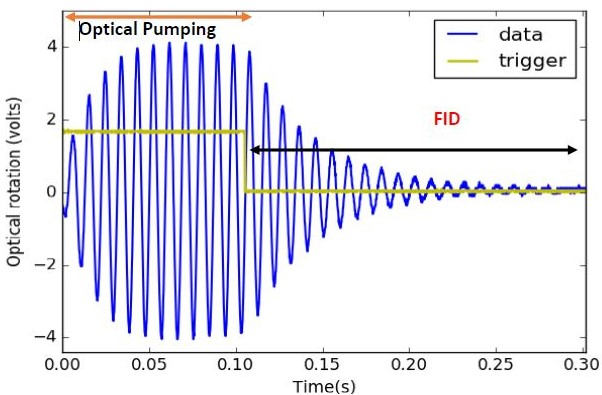
\includegraphics[width=0.55\linewidth]{figures/Capture2}
\caption{ An example of Free Induction Decay (FID) signal, when pumping the Rb atoms  was done for 0.1 s with linearly polarized light and probing was done for 0.2 s. The applied magnetic field during the measurement is $0.2~\mu T$. }
\end{figure}
The signal recorded  from X channel will be a sinusoid with an exponentially damping, according to   
  \begin{equation}
 y(t) = y_0 + A   e^{(t-t_0)/\tau}\sin(\omega t + \phi_0)\label{eq:decaying sinwave}
\end{equation}  

And the signal recorded  from Y channel will be a decaying cosine wave, according to
                                       
  \begin{equation}
 y(t) = y_0 + A   e^{(t-t_0)/\tau}\cos(\omega t + \phi_0)\label{eq:decaying coswave}
\end{equation}
where $y_0$ describes a possible offset, A is the maximum amplitude of the sinusoidal oscillation,
t the present time, $t_0$ the starting point of the measurement, $\omega$ the oscillation frequency and $\phi_0$  some possible phase shift. The data fitting procedure were done in two ways in order to study a variety of systematic effects that were encountered. One method is to take a least square fit of x and y data separately to a decaying sin and cosine wave respectively. Another way of data fitting is to fit X and Y data simultaneously. A least square-fit of the recorded data set to equation \ref{eq:decaying sinwave} or \ref{eq:decaying coswave} gives an estimate on frequency and  therefore the magnetic field.
\begin{figure}[h]
\centering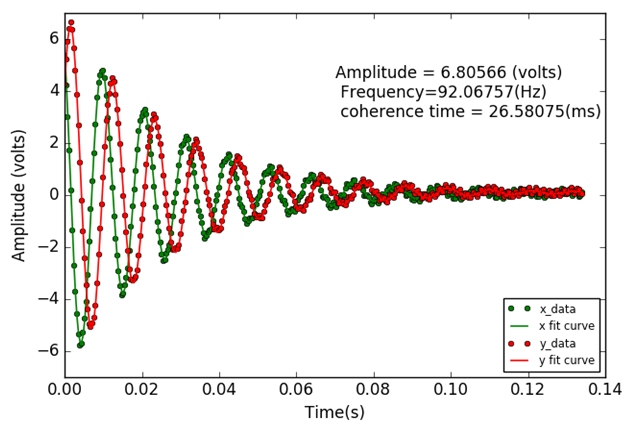
\includegraphics[width=0.55\linewidth]{figures/fid_simultaneous}
\caption{ Simultaneous fit of X and Y signal(green and red dots are represents x and y data respectively whereas green and red curve represents fit curves\label{Fig:FID fit}}
\end{figure}
  

The initial guesses for the least-square parameters are given
as:
\begin{itemize}
\item
Beat frequency $\omega$: In order to guess the beat frequency, the Fast Fourier Transform (FFT) of FID signal is done. The extracted FFT frequency is used as guess frequency.
\item
Amplitude A: In order to get guess amplitude, Averaging the maximum of the X and Y data is done.
\item
Offset $\phi_0$: The mean of FID signal is calculated. This mean value is used as guess for the offset. 

\end{itemize}
The data fitting procedure provides us the actual value for those parameters. The oscillation frequency, one of the extracted fit parameters, is then is used to estimate the magnetic field according to the following equation
\begin{equation}
 B= \frac{\nu_{fit}~ +~\nu_0}{2\gamma}\label{eq:field}
\end{equation}
 where $\nu_{fit}$ denotes the oscilation  frequency, $\nu_{0}$ is lock-in frequency and $\gamma$ is the gyromagnetic ratio of Rb vapor. Fig \ref{Fig:FID fit} shows an example least square fit of FID signal where both x and y output of lock-in has displayed.
 
Advantages: FID mode is free of  pump light induced frequency shifts or instabilities because the optical pumping is done for a very short time period and the frequency measurement takes place quickly. This frequency is later translate into magnetic field.\\ 

Disadvantages: As a finite duty cycle is used (pump modulation only happens during a short period of time and the main idea is to watch the coherence decay, a decreasing of the maximum achievable sensitivity with this method.



\subsection{FID in tilted magnetic field}
For the nEDM experiment it is very important to do tilted field measurement in order to have better understanding of  geometric phase effects which are the leading sources for systematic uncertainties during nEDM measurement . 
Since our Rb magnetometer is a scalar magnetometer, it is not possible to measure vector field components directly.In general, when the magnetic field is along the light propagation direction, the main resonance occurs at $\Omega_m = 2\Omega_L$. This resonance appear because of the symmetry of the optically pumped state. It is found that when magnetic field direction is tilted in the plane perpendicular to the light polarization axis, resonance is observed at  $\Omega_m = 2\Omega_L$~with its amplitude depending on the tilt angle. In this case, the amplitude of resonance signal decreases with increasing tilt angle . However, If we tilt the magnetic field direction towards the light polarization axis a new resonance appears at $\Omega_L$ along with the main resonance at $2\Omega_L$ if linearly polarized light is used. In this case the resonance signal contain two frequency component Fig \ref{fig:transverse} . The amplitude of the new resonance signal at $\Omega_L$  increases as the angle between B and the light propagation direction increases while main resonance amplitude at $2\Omega_L$  decrease with increasing tilt angle. However,when the tilt angle is larger than some certain angle the resonance amplitude measured at $\Omega_L$ also start to decrease and reaches zero when the magnetic field is directed along the y axis.   It could be possible to evaluate the magnitude of the magnetic field from the ratio of the resonance amplitudes at $\Omega_L$ and $2\Omega_L$. The same study with frequency modulated light has been reported by Pustelny et al.\cite{PhysRevA.74.063420}. In this study the NMOR Signal was observed by connecting the balanced photodiode to the oscilloscope directly. A python script is used to transfer the data presented on the oscilloscope screen to computer for further analysis. 

\begin{figure}
    \centering
 
    \begin{subfigure}[b]{0.45\textwidth}
        \centering
        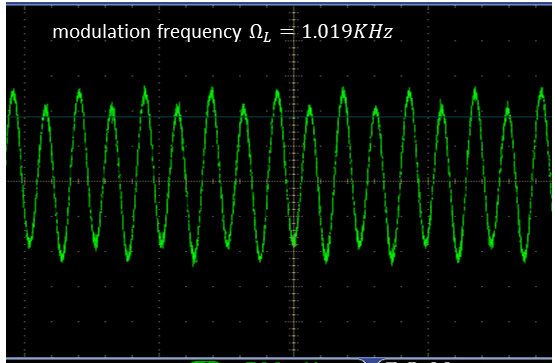
\includegraphics[width=\textwidth]{figures/transverse_field}
        \caption{}
        \label{fig:transverse}
    \end{subfigure}
    \hfill
    \begin{subfigure}[b]{0.45\textwidth}
        \centering
        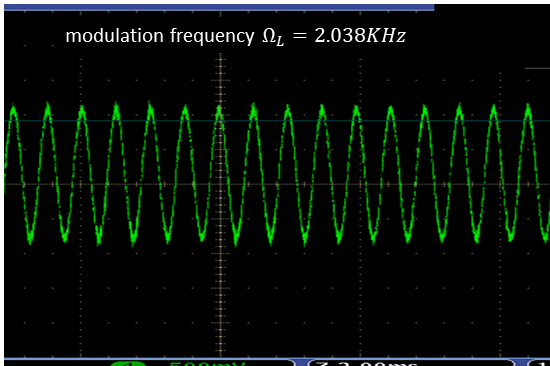
\includegraphics[width=\textwidth]{figures/transverse_field_2}
        \caption{}
        \label{fig:transverse2}
    \end{subfigure}
    \caption{(a) Optical rotation as a function of time at $\Omega_L$ in the yz plane at tilt angle $15\degree$ with light propagation direction. (b) Optical rotation as a function of time at $2\Omega_L$ for same tilt angle}
    \label{fig:Tilted field}
\end{figure}

